%% Outline
% 1. Navigation is important problem
% 1.5 Traditionally addressed by mapping during exploration and path
%      planning during exploitation.
% 2. End to end learning algorithms have shown promise to take over
%      mapping and path
% 3. We do not know how these algorithms work. There has been work in computer vision that shows the learning on neural network based methods can be learning totally different kind of patterns from what we would expect.
% 4.1 We find that it is not remembering the map it is being trained on
% 4.2 We find that no path planning is  happening only, memorizing and regeneration of the sequence of steps. However, it is not 

% 1. Navigation is important problem
% 1.5 Traditionally addressed by mapping during exploration and path
%      planning during exploitation.
Navigation remains a fundamental problems in mobile robotics and artificial intelligence~\cite{SmChIJRR1986,ElCOMPUTER1980}.
The problem is classically addressed by separating the eventual task of navigation into exploration, where the environment is represented in some sort of \emph{map} data-structure, and exploitation, where the map is used for localization and path-planning to find an optimal path to a given destination based on a given optimality criterion.  Although there have been many advances in this classical approach \cite{RaMoTaTROB2015,EnScCrECCV2014}, it remains a difficult challenge: for example, mapping errors propagate to localization and path-planning tasks; monocular navigation remains a challenge in textureless \cite{YaSoKaIROS2016} or repeated texture environments 

More recently, end-to-end navigation methods---methods that attempt to  
solve the navigation problem without breaking it down into separate parts of localization, mapping and path-planning---have gained traction.
%
% 2. End to end learning algorithms have shown promise to take over
%      mapping and path-planning
With the recent success of Deep Reinforcement Learning (DRL) \cite{MnKaSiNATURE2015}, these end-to-end navigation methods \cite{MnBaMiICML2016,SiHuMaNATURE2016,LePaKrISER2017,MiPaViICLR2017,OhChSiICML2016} forego decisions about the details that are required in the intermediate step of mapping.
The potential for simpler yet capable methods is rich; for example, one can optimize to store only the minimal amount of map information that is required to optimally perform the end task of navigation.
One such method \cite{MiPaViICLR2017} has recently shown promise of navigation using only first person monocular view in randomly generated mazes. Not only their algorithm shows evidence of localization, but they also show some of evidence of better than random path planning when the goal location is randomly chosen during evaluation time. 

\begin{figure}
%\rotatebox{90}{\hspace{3em}Trained on 1 map }
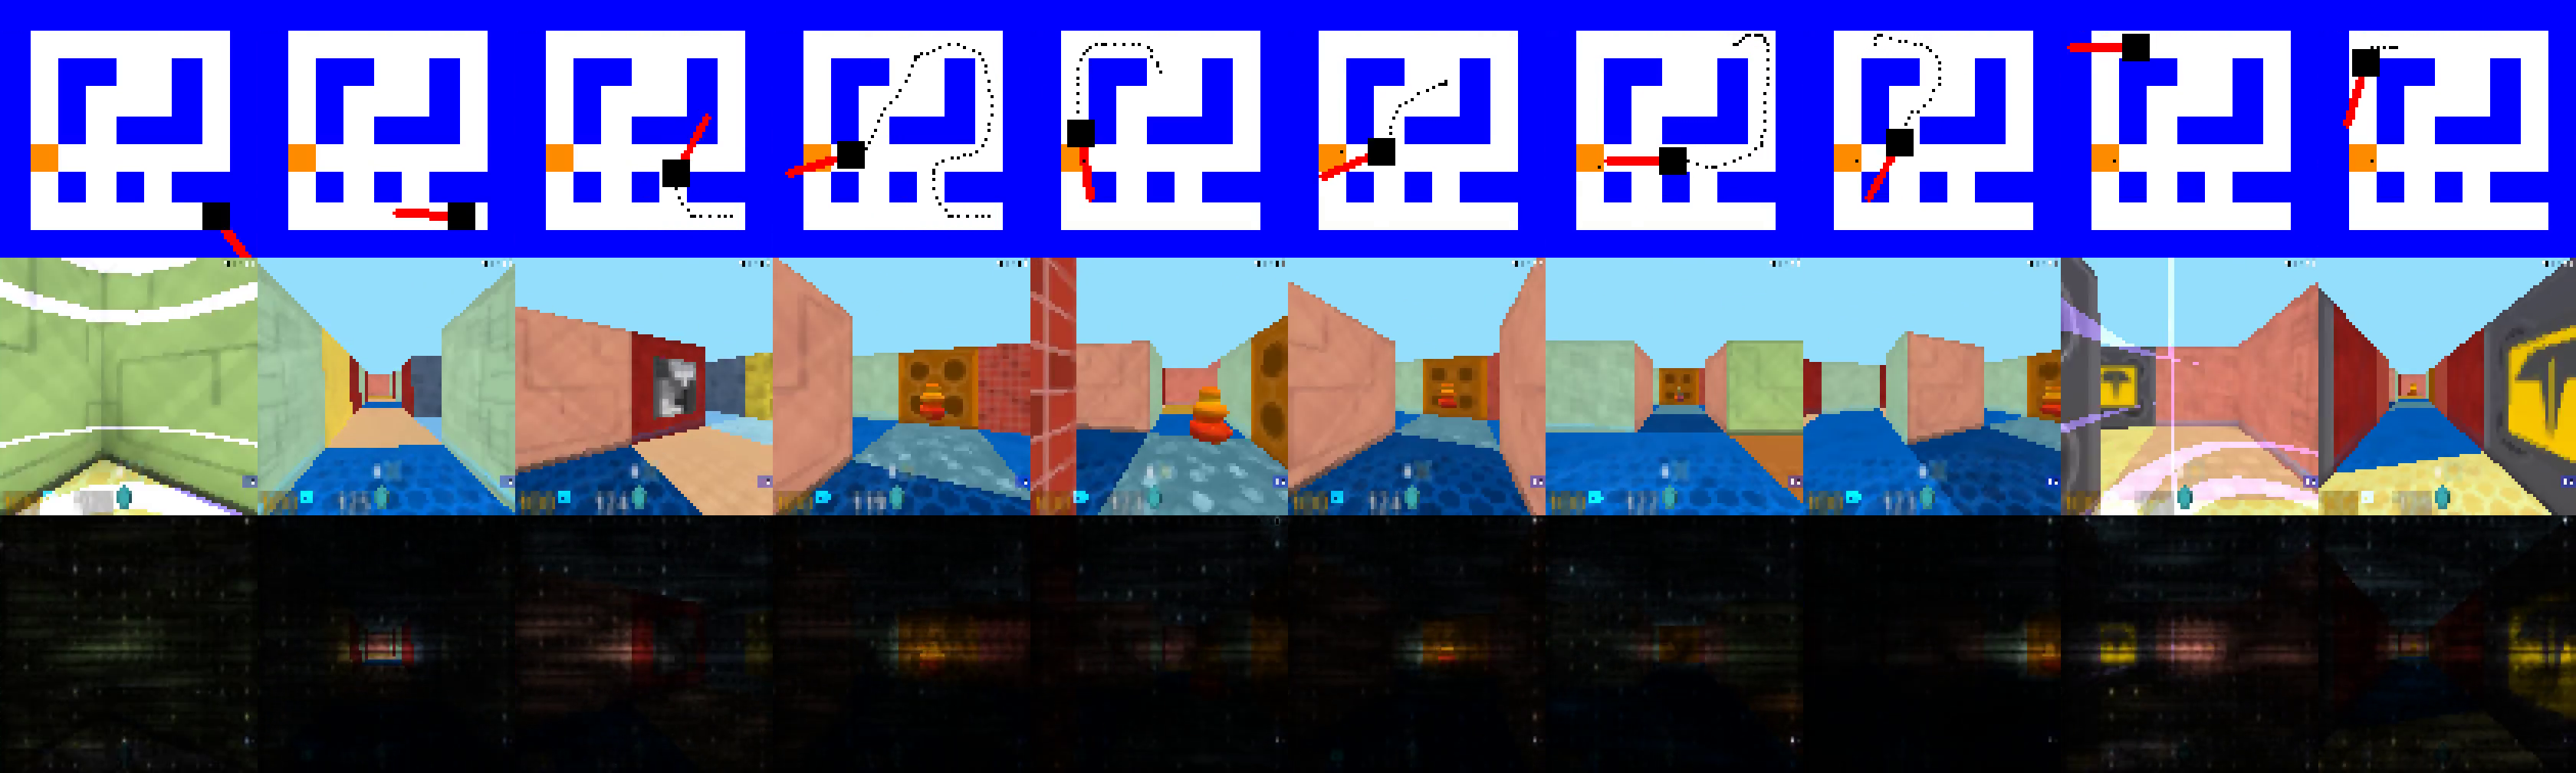
\includegraphics[width=\textwidth]{./exp-results/training-09x09-0127-on-0127.png}
%\rotatebox{90}{\hspace{2em}Trained on 1000 maps }
%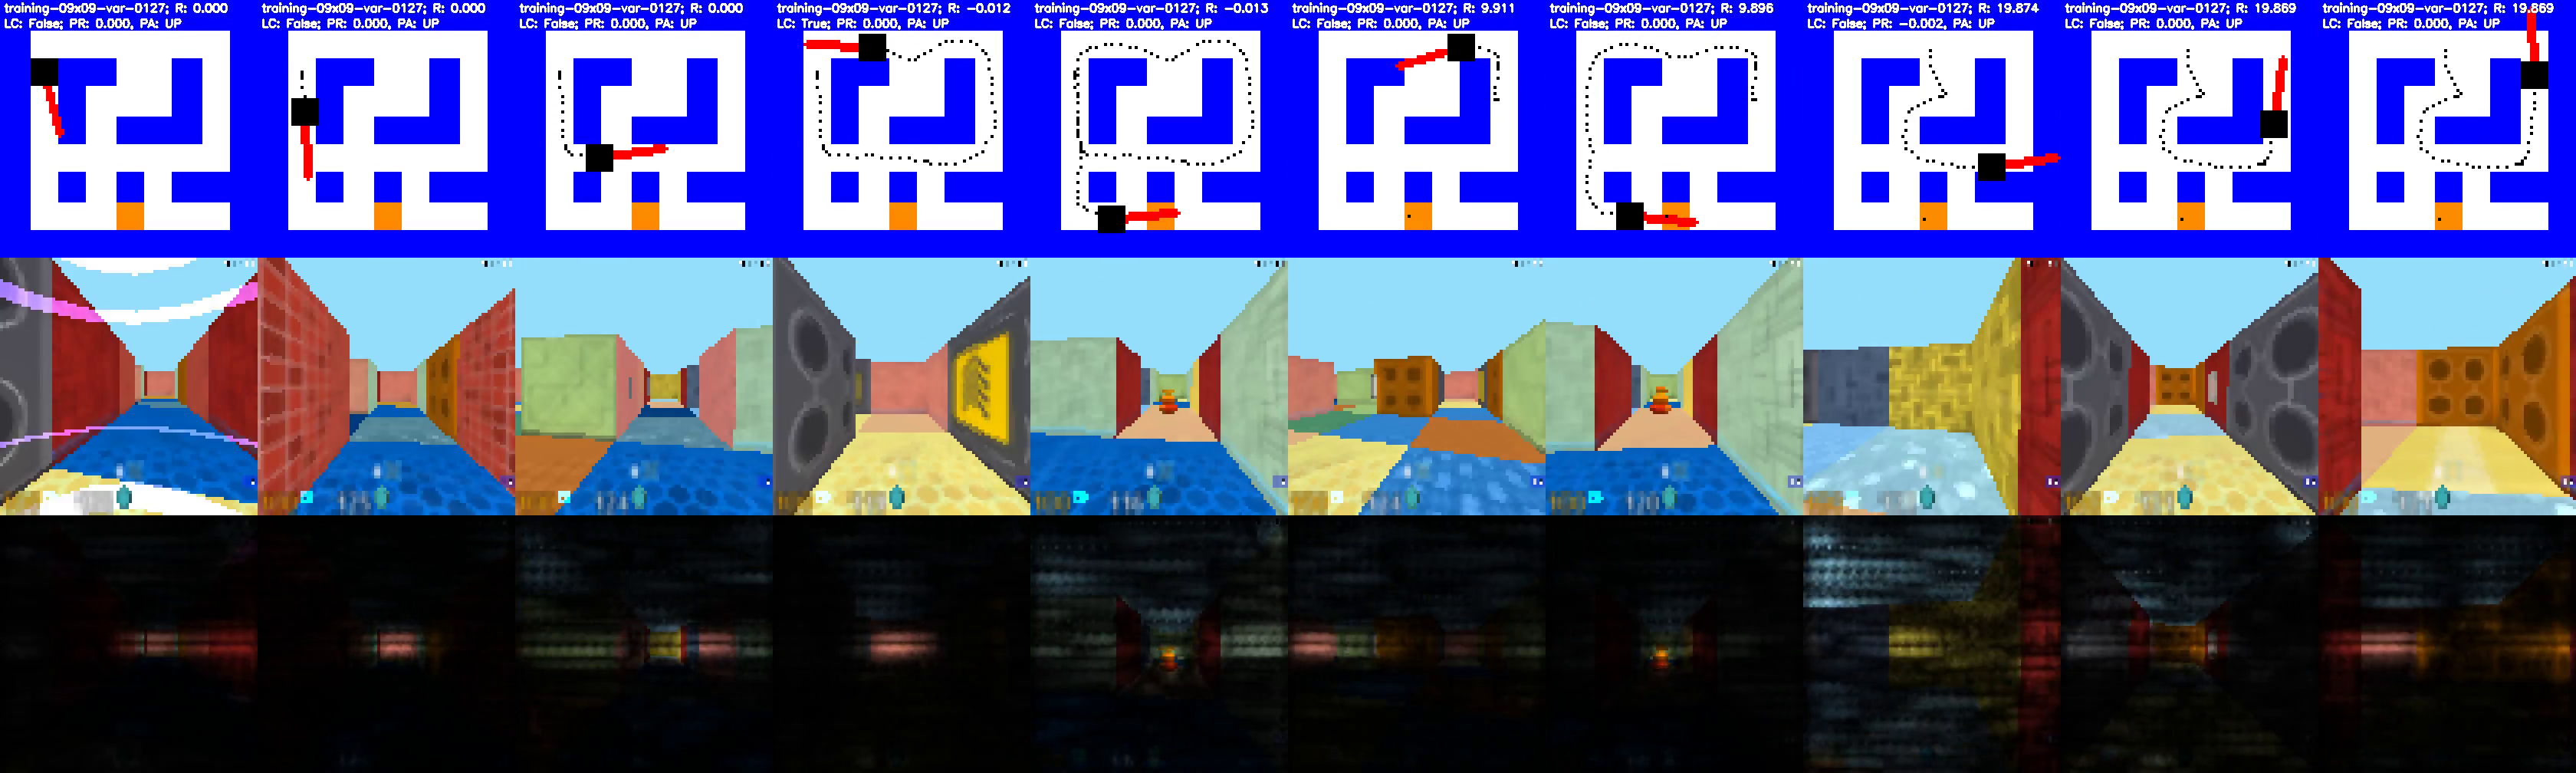
\includegraphics[width=\textwidth]{./exp-results/training-1000-on-0127.png}
\caption{Qualitative results of evaluating algorithm on map id 127. The top three rows show selected frames for the algorithm trained on the same map 127, while the bottom three rows show the result of evaluting the algorithm trained on 1000 maps evaluated on 127. The top row shows the top view of the robot moving through the maze, second row shows the first person which is the only input available to the agent (except reward). The third row shows the attention masked view of the algorithm. We observe that the algorithm focuses attention at the horizon in long corridors, on the goal object (it looks like stacked rings) and on interesting decals.}
\label{fig:training-qualitative}
\end{figure}

% 3. We do not know how these algorithms work. There has been work in computer vision that shows the learning on neural network based methods can be learning totally different kind of patterns from what we would expect.
Despite this potential and recent successes, 
state-of-the-art DRL based methods have been confronted with their own set of problems, such as difficulty to understand the method limitations or the kind of patterns the algorithm is understanding.  The black-box nature of these methods make them hard to study.
On similar lines, \cite{NgYoClCVPR2015} show that neural-network-based object detection methods can be easily fooled by introducing noise that is imperceptible to humans. Hence, it is important to analyze the DRL methods to understand if they are truly ``learning to navigate'' \cite{MiPaViICLR2017}.

% 4.1 We find that it is not remembering the map it is being trained on
% 4.2 We find that no path planning is  happening only, memorizing and regeneration of the sequence of steps. However, it is not 

In this work, we focus on the work of \cite{MiPaViICLR2017} and analyze the method using multiple random maps with different degrees of randomness. As a generalization, we propose a 4-stage benchmark for end-to-end navigation methods.
Our experimental setup is similar to \cite{MiPaViICLR2017} and uses the same open source library Deepmind's Lab \cite{BeLeTeARXIV2016}.
We setup a maze where the goal is randomly placed and the agent is randomly spawned.
The objective of the agent is to hit the goal as many times as possible within a fixed episode time.
Every time the agent hits the goal, it respawns at a random location.
With this setup \cite{MiPaViICLR2017} found that the agent finds the goal faster the second time onwards as compared to the first time.
This implies that agent is somehow able to exploit the new information about position of the goal to reach the goal faster.
However, \cite{MiPaViICLR2017} do not rule out random chance because they only show the successful result on random goal case with only one map, do not report standard deviation on their metrics and do not evaluate the algorithm on unseen maps.
Even though separting training and testing sets is the obvious thing to do in machine learning, we are the first work to evaluate any DRL based navigation method on unseen maps.
We expand on their analysis and evaluate the same metric on multiple types of maps including randomly generated maps.

We find no evidence of DRL agents being able to perform shortest path-planning in unseen mazes even in simple mazes.
We observe that the agent prefers to take a particular path just as an artifact of initialization.
We hypothesize that the agents are learning a correspondence between local sequence of frames and actions.
These findings are the results on testing and training on multiple maps that were randomly chosen from set of 1100 randomly generated maps.
We provide thorough and clear summary data to substantiate these findings as well as individual maps and results to explain them carefully.
A secondary finding is that even if the agent is trained on a single maze it is able to navigate better than random in unseen mazes.

